\matlab is a popular numeric programming language, used by millions of
scientists, engineers as well as students worldwide\cite{MatlabGrowth}.  \matlab
programmers appreciate the high-level matrix operators,  the fact that
variables and types do not need to be declared, the large number of library and
builtin functions available, and the interactive style of program development
available through the IDE and the interpreter-style read-eval-print loop.
However, even though \matlab programmers appreciate all of the features that
enable rapid prototyping,  their applications are often quite compute intensive
and time consuming. These applications could perform much more efficiently if
they could be easily ported to a high performance computing system.  

On the other hand, \xten is an object-oriented and statically-typed language
which uses cilk-style arrays indexed by \emph{Point} objects, and has been
designed with well-defined semantics and high performance computing in mind.
\xten compiler can generate C++ or Java code and supports various communication
interfaces including sockets and MPI for communication between nodes on a
parallel computing system.

In this thesis we present \mixten, a source-to-source compiler that helps
to bridge the gap between \matlab, a language familiar to scientists,
and \xten,  a language designed for high performance computing systems. 
\mixten statically compiles \matlab programs to \xten and thus
allows scientists and engineers to write programs in \matlab (or use old 
programs already written in \matlab) and still get the benefits of high 
performance computing without having to learn a new language. Also, systems that
use \matlab for prototyping and C++ or Java for production, can benefit from
\mixten by quickly converting \matlab prototypes to C++ or Java programs via 
\xten. \figref{Fig:flow} shows the flow of compilation from \matlab to
executable code via \mixten. In particular, this thesis identifies the key 
challenges in compiling a
dynamically-typed language like \matlab to a statically-typed object-orinted
high performance computing language like \xten and our approach to 
compiling \matlab to \xten.
\begin{figure}[htbp]                                                            
\begin{center}                                                                  
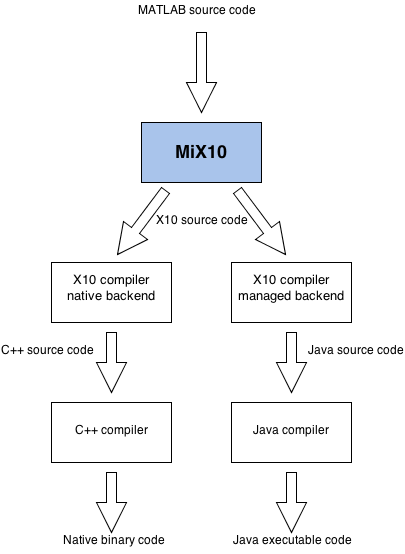
\includegraphics[scale=0.4]{images/mix10_compilation_flow}                             
\caption {Compilation flow via \mixten}\label{Fig:flow}                    
\end{center}                                                                    
\end{figure}     

On one hand, all the aforementioned characteristics of \matlab make it a very 
user-friendly and thus popular application to develop software among a
non-programmer community. On the other hand, these same characteristics make
\matlab a difficult language to write a static compiler for. Lack of formal 
language specification, unconventional semantics and closed source make compiler
writers' task even harder. Mathworks implementation of \matlab is essentially an
interpreter with a \emph{JIT accelarator} which is generally slower than statically
compiled languages. Built on top of \mclab frontend and static analysis tools,
 \mixten provides static compilation for \matlab via the C++
backend for \xten and thus ultimately aims to have better performance even with
sequential code. 
%uncomment below if tamer+ used
%\mixten also concentrates on readability of the generated \xten
%code to meet the other goal of this thesis, which is to help users port 
%their code from \matlab to \xten.    

\section{Contributions}
  
The major contributions  of this thesis are as follows:

\begin{description}

\item[Identifying key challenges:] We have identified the key challenges
in performing a semantics-preserving translation of \matlab to \xten.

\item[Overall design of \mixten:] We provide the design of a 
source-to-source translator, building upon the McLab front-end and
analysis toolkits.

\item[\mixten IR design:] In order to provide a convenient
target for the first level of translation, we have defined a high-level
\mixten IR.  This IR is used for code generation, \xten specific analyses, 
code simplifications and transformations.

\item[Comparison of different kinds of \xten arrays:] version 2.4 of \xten 
(latest version as of this writing) provides two kinds of multi-dimensional 
arrays, \emph{region-based} arrays and \emph{rail-backed} arrays.  

\item[Static analyses:] We developed various static analyses to aid generation
of better optimized code and to support wider range of \matlab functionalities.
Identification of complex numerical values, handling variables with	
type-conflicts, array-bounds checks and identification of non-mutable variables
are the important analyses that we describe in this thesis.

\item[Template-based builtin framework:] \matlab supports many builtin
operations that can operate over a wide variety of run-time types.  We
have designed and implemented a template-based system that allows us to
generate specialized \xten code for a collection of important builtin
operations.

\item[Code generation strategies for key language constructs:]  There
are some very significant differences between the semantics of \matlab
and \xten.  A key difference is that \matlab is dynamically-typed,
whereas \xten is statically-typed.   Furthermore, the type rules are
quite different, which means that the generated \xten code must include
the appropriate explicit type conversion rules, so as to match the
\matlab semantics.   Other \matlab features, such as multiple returns
from functions, a non-standard semantics for \texttt{for} loops, and a
very general range operator, must also be handled correctly.

\item[Working implementation and performance results:] We have implemented the 
\mixten compiler over various \matlab compiler tools provided by \mclab. In the
process we also implemented some enhancements to these existing tools.
We provide performance results for different \xten backends over a set 
of benchmarks and compare them with results from other \matlab compilers
including Mathworks \matlab implementation and Octave.

\end{description}

\section{Thesis Outline}

This thesis is divided into \ref{chap:Conclusions} chapters, including this one
and is structured as follows. 

\chapref{chap:Xten} provides an introduction to the \xten language and describes
how it compares to \matlab from the point of view of language design.
\chapref{chap:Background} gives a description of various existing \matlab
compiler tools upon which \mixten is implemented. 
\chapref{chap:Design} gives a high-level design of \mixten and explains the
design and need of \mixten IR.
In \chapref{chap:Arrays} we introduce different types of arrays provided by
\xten and describe code generation strategies for them. We also identify pros
and cons of both kinds of arrays in the context of \xten as a target language.
\chapref{chap:Builtin} presents the template-based specialization framework for
handling \matlab builtin methods.
\chapref{chap:Analyses} describes the various static analyses that we
implemented to help generate more optimized code.
In \chapref{chap:Codegen} we give details of code generation strategies for
important \matlab constructs.
\chapref{chap:Evaluation} provides performance results for code generated using
\mixten for a suite of benchmarks.
\chapref{chap:Related} provides an overview of related work and
\chapref{chap:Conclusions} concludes and outlines possible future work.

